\chapter{Geometric planetary orbit models}\label{ckep}
% !TEX root = ./Almagest.tex

\section{The model of Kepler}
In this chapter, 
 Kepler's geometric model of  a geocentric planetary orbit is  examined in detail, and then compared to the 
less accurate geometric models of Hipparchus, Ptolemy, and Copernicus. In the following,
all orbits are viewed from the  northern ecliptic pole.

Kepler's geometric model of a heliocentric planetary orbit is summed up in his   three well-known laws of planetary motion.
According to Kepler's first law, all planetary orbits are ellipses  that are  confocal with the Sun and lie in a
fixed plane.
Moreover, according to Kepler's second law, the radius vector which connects the Sun to a given planet sweeps out  equal areas in equal time intervals. 

\begin{figure}[h]
\centerline{\includegraphics[height=2.in]{Fig4-1.eps}}
\caption{A Keplerian orbit.}\label{jf1}
\end{figure}

Consider Figure~\ref{jf1}. The curve $\Pi PBA$ is half  of an elliptical planetary orbit. Furthermore, $C$ is the
geometric center of the orbit, $S$ the focus at which the Sun is located,
$P$ the instantaneous position of the planet, $\Pi$ the perihelion point (that is, the planet's point of closest approach to the Sun),
and $A$ the aphelion point (that is, the  point of furthest distance from the Sun). The ellipse is symmetric about
$\Pi A$, which is termed the {\em major axis}, and about $CB$,
which is termed the {\em minor axis}.
The length $CA\equiv a$ is called the orbital
{\em major radius}. The length $CS$  represents the displacement of the Sun from
the geometric center of the orbit, and is generally written $e\,a$, where $e$ is termed the
orbital {\em eccentricity}, and $0\leq e\leq 1$. The length $CB\equiv b = a\,(1-e^2)^{1/2}$ is called
the orbital {\em minor radius}. 
The length $SP\equiv r$ represents the radial distance of the planet from the Sun.
Finally, the angle $RSP\equiv T$ is the angular bearing of the planet from the Sun,
relative to the major axis of the orbit, and is termed the {\em true anomaly}. 

The curve $\Pi QDA$ is half of a circle whose geometric center is $C$, and whose
radius is $a$. Hence, the circle passes through the perihelion and aphelion
points. $R$ is the point at which the perpendicular from $P$ 
meets the major axis $\Pi A$. The point where $RP$ produced
meets circle $\Pi QDA$ is denoted $Q$. Finally,
the angle $SCQ\equiv E$ is called the {\em elliptic anomaly}. 

Now, the equation of the ellipse $\Pi PBA$ is
\begin{equation}
\frac{x^2}{a^2}+ \frac{y^2}{b^2} = 1,
\end{equation}
where $x$ and $y$ are the perpendicular distances from the minor and major
axes, respectively. Likewise, the equation of the circle $\Pi QDA$ is
\begin{equation}
\frac{x'^{\,2}}{a^2} + \frac{y'^{\,2}}{a^2} = 1.
\end{equation}
Hence, if $x=x'$ then
\begin{equation}
\frac{y}{y'} = \frac{b}{a},
\end{equation}
and it follows that
\begin{equation}\label{je4}
\frac{RP}{RQ} = \frac{b}{a}.
\end{equation}

Now, $CS = e\,a$. Furthermore, it is easily demonstrated that
 $SR=r\,\cos T$, $RP=r\,\sin T$, $CR= a\,\cos E$, and $RQ= a\,\sin E$. Consequently, Equation~(\ref{je4}) yields
\begin{equation}\label{je5}
r\,\sin T = b\,\sin E = a\,(1-e^2)^{1/2}\,\sin E.
\end{equation}
Also, because $SR = CR-CS$, we have
\begin{equation}\label{je6}
r\,\cos T = a\,(\cos E - e).
\end{equation}
Taking the square root of the sum of the squares of the previous two equations, we obtain
\begin{equation}\label{je7}
r = a\,(1-e\,\cos E),
\end{equation}
which can be combined with Equation~(\ref{je6}) to give
\begin{equation}
\cos T = \frac{\cos E - e}{1-e\,\cos E}.
\end{equation}

Now, according to Kepler's second law,
\begin{equation}
\frac{{\rm Area}\,\Pi PS}{\pi\,a\,b} = \frac{t-t_\ast}{\tau},
\end{equation}
where $t$ is the time at which the planet passes point $P$,  $t_\ast$  the time at which it passes the perihelion point,
and $\tau$ the {\em orbital period}.
However,
\begin{align}
{\rm Area}  \,\Pi PS &= {\rm Area}\, SRP + {\rm Area} \,\Pi RP
= \frac{1}{2}\,r^2\,\cos T\,\sin T + {\rm Area}\,\Pi RP.
\end{align}
But,
\begin{equation}
{\rm Area}\,\Pi RP = \frac{b}{a}\,{\rm Area}\,\Pi RQ,
\end{equation}
because $RP/RQ = b/a$ for all values of $T$. In addition, 
\begin{align}
{\rm Area}\,\Pi RQ = {\rm Area}\,\Pi QC - {\rm Area}\,RQC= \frac{1}{2}\,E\,a^2 - \frac{1}{2}\,a^2\,\cos E\,\sin E.
\end{align}
Hence, we can write
\begin{equation}
\left(\frac{t-t_\ast}{\tau}\right) \pi\,a\,b= \frac{1}{2}\,r^2\,\cos T\,\sin T + \frac{b}{a}\,\frac{a^2}{2}\,(E - \cos E\,\sin E).
\end{equation}
According to Equations~(\ref{je5}) and (\ref{je6}), $r\,\sin T = b\,\sin E$, and $r\,\cos T = a\,(\cos E - e)$, so
the previous expression reduces to
\begin{equation}
M = E - e\,\sin E,
\end{equation}
where
\begin{equation}
M = \left(\frac{2\pi}{\tau}\right)\,(t-t_\ast)
\end{equation}
is an angle that is zero at the perihelion point, increases  uniformly in time, and has a repetition period that 
matches the period of the planetary orbit. This angle is termed the {\em mean anomaly}. 

In summary, the radial and angular polar coordinates, $r$ and $T$, respectively,
of a planet in a Keplerian orbit about the Sun are specified as  implicit functions
of the mean anomaly, which is a  linear function of time, by the
following three equations:
\begin{align}
M &= E - e\,\sin E,\\[0.5ex]
r &= a\,(1- e\,\cos E),\\[0.5ex]
\cos T &= \frac{\cos E - e}{1-e\,\cos E}.
\end{align}
It turns out that the Earth and the five visible (to the naked eye) planets all possess  low eccentricity orbits characterized by $0<e\ll 1$. Hence, it is a good approximation to expand the previous three equations
using $e$ as a small parameter. To second order, we
get
\begin{align}
E &= M + e\,\sin M + (1/2)\,e^2\,\sin 2M,\\[0.5ex]
r& = a\,(1-e\,\cos T - e^2\,\sin^2 T),\\[0.5ex]
T &= E + e\,\sin E + (1/4)\,e^2\,\sin 2 E.
\end{align}
Finally, these equations can be combined to give $r$ and $T$ as explicit  functions of the
mean anomaly:
\begin{align}
\frac{r}{a} &= 1 -e\,\cos M + e^2\,\sin^2 M,\label{je22}\\[0.5ex]
T &= M + 2\,e\,\sin M + (5/4)\,e^2\,\sin 2M.\label{je23}
\end{align}

\section{The model of Hipparchus}
Hipparchus's geometric model of the apparent orbit of the Sun around the Earth can also be used to describe a heliocentric planetary orbit. The model is illustrated  in Figure~\ref{hipp}. The orbit of the planet corresponds
to the circle $\Pi P D A$ (only half of which is shown), where $\Pi$ is the perihelion point, $P$ the planet's instantaneous position,
and $A$ the aphelion point. The diameter $\Pi   S C A$ is the effective major axis of the orbit (to be more exact, it
is the line of apsides), where $C$ is the geometric center of circle $\Pi P D A$, and $S$ the fixed position of the Sun.
The radius $CP$ of circle $\Pi PDA$ is   the effective major radius, $a$, of the orbit.  The distance $SC$ is
equal to $2\,e\,a$, where $e$ is the orbit's effective eccentricity. The angle $PC\Pi$
is  identified with the  mean anomaly, $M$, and increases  linearly  in time.  In other words, as seen from $C$, the planet
$P$ moves  uniformly around circle $\Pi PDA$ in a counterclockwise direction. Finally, $SP$ is the radial
distance, $r$, of the planet from the Sun, and angle $P S \Pi$ is the planet's true anomaly, $T$.

\begin{figure}[h]
\centerline{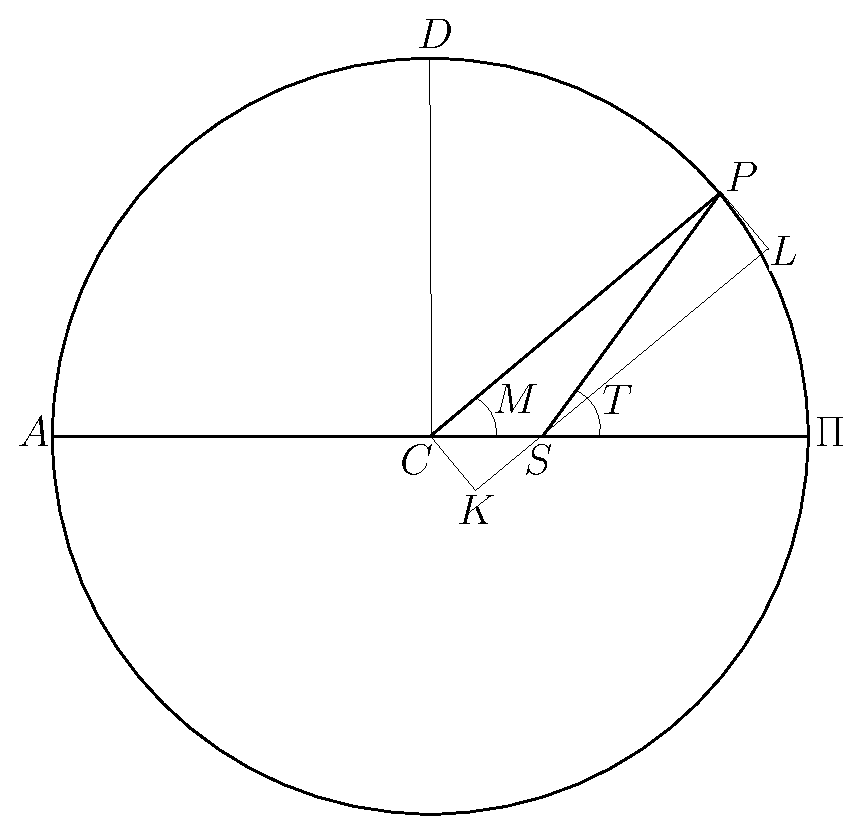
\includegraphics[height=2.5in]{Fig4-2.eps}}
\caption{A Hipparchian orbit.}\label{hipp}
\end{figure}

Let us draw the straight-line $KSL$ parallel to $CP$, and passing through point $S$, and then complete the rectangle $PCKL$. Simple geometry reveals that 
$CK = PL = 2\,e\,a\,\sin M$, $KS=2\,e\,a\,\cos M$, and  $SL = a-2\,e\,a\,\cos M$. Moreover, according to the theorem of Pythagoras, $SP^2 = SL^2+ PL^2$,
which implies that
\begin{equation}
\frac{r}{a} = (1-4\,e\,\cos M + 4\,e^2)^{1/2}.
\end{equation}
Now, $T = M + q$, where $q$ is angle $PSL$. However,
\begin{equation}
\sin q = \frac{PL}{SP} = \frac{2\,e\,\sin M}{(1-4\,e\,\cos M + 4\,e^2)^{1/2}}.
\end{equation}

Finally, expanding the previous two equations to second order in the small parameter $e$, we obtain
\begin{align}\label{e4.26}
\frac{r}{a} &= 1 -2\,e\,\cos M + 2\,e^2\,\sin^2 M,\\[0.5ex]
T &= M + 2\,e\,\sin M + 2\,e^2\,\sin 2M.\label{e4.27}
\end{align}
It can be seen, by comparison with Equations~(\ref{je22}) and (\ref{je23}), that   the relative radial distance, $r/a$, in the Hipparchian model deviates from that in the (correct) Keplerian model to  first order in $e$ (in fact, the variation of $r/a$
is greater by a factor of two in the former model), whereas 
 the true anomaly, $T$,  only deviates  to  second order  in $e$.  We conclude that  Hipparchus's geometric model
 of a heliocentric planetary orbit does a
 reasonably good job at predicting the angular position of the planet, relative to the Sun, but significantly
 exaggerates (by a factor of two) the variation in the radial distance between the two during the course of a complete  orbital rotation. 

\section{The model of Ptolemy}
Ptolemy's geometric model of the motion of the center of an epicycle around a deferent can also be used to describe a heliocentric planetary orbit. The model is illustrated  in Figure~\ref{ptol}. The orbit of the planet corresponds
to the circle $\Pi P D A$ (only half of which is shown), where $\Pi$ is the perihelion point, $P$ the planet's instantaneous position,
and $A$ the aphelion point. The diameter $\Pi   S C Q A$ is the effective major axis of the orbit, where $C$ is the geometric center of circle $\Pi P D A$,  $S$ the fixed position of the Sun, and $Q$  the location of the so-called {\em equant}.
The radius $CP$ of circle $\Pi PDA$ is   the effective major radius, $a$, of the orbit.  The distances $SC$ and $CQ$ are both
equal to $e\,a$, where $e$ is the orbit's effective eccentricity. The angle $PQ\Pi$
is  identified with the  mean anomaly, $M$, and increases linearly  in time.  In other words, as seen from $Q$, the planet
$P$ moves uniformly  around circle $\Pi PDA$ in a counterclockwise direction. Finally, $SP$ is the radial
distance, $r$, of the planet from the Sun, and angle $P S \Pi$ is the planet's true anomaly, $T$.

\begin{figure}[h]
\centerline{\includegraphics[height=2.5in]{Fig4-3.eps}}
\caption{A Ptolemaic orbit.}\label{ptol}
\end{figure}

Let us draw the straight-line $KSL$ parallel to $QP$, and passing through point $S$, and then complete the rectangle $PQKL$. Simple geometry reveals that 
$QK = PL = 2\,e\,a\,\sin M$, $KS=2\,e\,a\,\cos M$, and  $SL = \rho-2\,e\,a\,\cos M$, where
$\rho=QP$. The cosine rule applied to triangle $CQP$ yields
$CP^2 = CQ^2+QP^2-2\,CQ\,QP\,\cos M$, or $\rho^2-2\,e\,a\,\cos M\,\rho -a^2\,(1-e^2)=0$, which
can be solved to give $\rho/a = e\,\cos M +(1-e^2\,\sin^2 M)^{1/2}$. 
 Moreover, according to the theorem of Pythagoras,  $SP^2 = SL^2+ PL^2$,
which implies that
\begin{equation}\label{e4.30x}
\frac{r}{a} = [1-2\,e\,\cos M\,(1-e^2\,\sin^2 M)^{1/2}+e^2+2\,e^2\,\sin^2 M]^{1/2}.
\end{equation}
Now, $T = M + q$, where $q$ is angle $PSL$. However,
\begin{equation}\label{e4.31x}
\sin q = \frac{PL}{SP} = \frac{2\,e\,\sin M}{[1-2\,e\,\cos M\,(1-e^2\,\sin^2 M)^{1/2}+e^2+2\,e^2\,\sin^2 M]^{1/2}}.
\end{equation}

Finally, expanding the previous two equations to second order in the small parameter $e$, we obtain
\begin{align}
\frac{r}{a} &= 1 -e\,\cos M + (3/2)\,e^2\,\sin^2 M,\label{e4.30}\\[0.5ex]
T &= M + 2\,e\,\sin M + e^2\,\sin 2M.\label{e4.31}
\end{align}
It can be seen, by comparison with Equations~(\ref{je22})--(\ref{je23}) and (\ref{e4.26})--(\ref{e4.27}), that   Ptolemy's geometric model of a heliocentric planetary orbit is significantly
more accurate than  Hipparchus's model, because the 
relative radial distance, $r/a$,  and the true anomaly, $T$, in the former model both only deviate from those in the (correct) Keplerian model to second order in $e$.

\section{The model of Copernicus}
Copernicus's geometric model of  a heliocentric planetary orbit is illustrated  in Figure~\ref{cop}. 
The planet $P$ rotates on a circular epicycle $YP$ whose center $X$ moves around the Sun on the eccentric circle $\Pi X D A$ (only
half of which is shown). The diameter $\Pi S C A$ is the effective major axis of the orbit, where $C$ is the geometric center of circle $\Pi X D A$,  and $S$ the fixed position of the Sun. When $X$ is at  $\Pi$ or $A$ the planet is at its perihelion
or aphelion points, respectively.  The radius $CX$ of circle $\Pi XDA$ is   the effective major radius, $a$, of the orbit.  The distance $SC$ is
equal to $(3/2)\,e\,a$, where $e$ is the orbit's effective eccentricity. Moreover, the radius $XP$ of the epicycle is equal to $(1/2)\,e\,a$. 
The angle $XC\Pi$
is  identified with the  mean anomaly, $M$, and increases linearly   in time.  In other words, as seen from $C$, the center of
the epicycle
$X$ moves  uniformly  around circle $\Pi XDA$ in a counterclockwise direction. The angle $PXY$, where $Y$ is
point at which $CX$ produced meets the epicycle,  is equal to
the mean anomaly $M$. In other words, the planet $P$ moves  uniformly around the epicycle $YP$, in an counterclockwise direction, at  twice 
the speed that point $X$ moves around circle $\Pi XDA$.
 Finally, $SP$ is the radial
distance, $r$, of the planet from the Sun, and angle $P S \Pi$ is the planet's true anomaly, $T$.

\begin{figure}[h]
\centerline{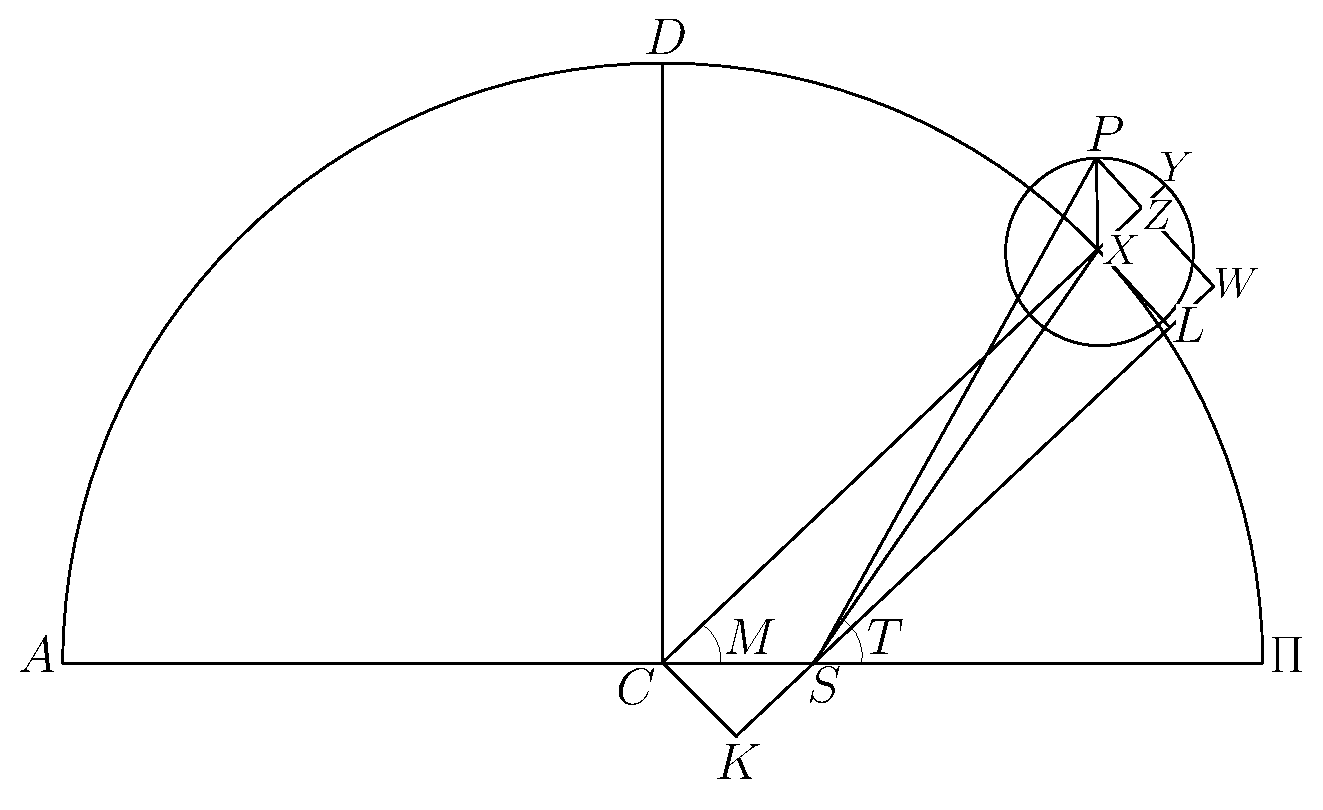
\includegraphics[height=2.5in]{Fig4-4.eps}}
\caption{A Copernican orbit.}\label{cop}
\end{figure}

Let us draw the straight-line $KSL$ parallel to $CX$, and passing through point $S$, and then complete the rectangle $XCKL$. Simple geometry reveals that 
$CK = XL = (3/2)\,e\,a\,\sin M$, $KS=(3/2)\,e\,a\,\cos M$, and  $SL = a-(3/2)\,e\,a\,\cos M$. Let $PZ$ be drawn normal
to $XY$, and let it meet $KSL$ produced at point $W$. Simple geometry reveals that $ZW=XL$,  $ZP=(1/2)\,e\,a\,\sin M$, and $XZ =LW = (1/2)\,e\,a\,\cos M$. It follows that $WP = ZW+ZP = XL+ZP = 2\,e\,a\,\sin M$, and $SW = SL+LW=SL+XZ= a-e\,a\,\cos\,M$.
Moreover, according to the theorem of Pythagoras,  $SP^2 = SW^2+ WP^2$,
which implies that
\begin{equation}
\frac{r}{a} = (1-2\,e\,\cos M +e^2+3\,e^2\,\sin^2 M)^{1/2}.
\end{equation}
Now, $T = M + q$, where $q$ is angle $PSW$. However,
\begin{equation}
\sin q = \frac{WP}{SP} = \frac{2\,e\,\sin M}{(1-2\,e\,\cos M +e^2+3\,e^2\,\sin^2 M)^{1/2}}.
\end{equation}

Finally, expanding the previous two equations to second order in the small parameter $e$, we obtain
\begin{align}
\frac{r}{a} &= 1 -e\,\cos M + 2\,e^2\,\sin^2 M,\\[0.5ex]
T &= M + 2\,e\,\sin M + e^2\,\sin 2M.
\end{align}
It can be seen, by comparison with Equations~(\ref{je22})--(\ref{je23}) and (\ref{e4.30})--(\ref{e4.31}), that, as is the case for Ptolemy's  model, both the 
relative radial distance, $r/a$,  and the true anomaly, $T$, in Copernicus's geometric model of a heliocentric planetary orbit only deviate from those in the (correct) Keplerian model to  second order  in $e$. However, the deviation  in the Ptolemaic
model is  slightly smaller  than that in the Copernican model. To be more exact, the maximum deviation in $r/a$
is $(1/2)\,e^2$ in the former model, and $e^2$ in the latter. On the other hand, the maximum deviation in $T$ is $(1/4)\,e^2$
in both models.